%--------------------------------------------------------------------------------
% 
\chapter{Evaluation}
\label{chapter:evaluation}
%--------------------------------------------------------------------------------

Validation of the proposed approach was performed using our \emph{Curious Cat}
implementation of the proposed KA approach, running alive over the course of 4 
years engaging a total of 728 registered 
users (users which are part of the experiment. Overall the implementation have
some additional users). During that time, the users checked-into 5,551 locations
and responded 
to 57,978 questions, out of which 8,611 were voting questions (7,560 positive 
and 1,051 negative votes), 18,907 questions were answered with "I don't know", 
and 30,460 real answers was inserted into the KB as new knowledge, including 
31,140 concepts (3,171 connected to instances of $User$ concept, 22,563 
check-ins and other places, and 5,406 other concepts). 
These triggered additional 386,980 assertions to be added through 
forward-chained inference. These can be separated into facts (374,300 
assertions) and additional derived question generating rules and questions 
(12,680). Altogether we gathered \textbf{444,958 (374,300 + 30,460)} pieces of 
completely new knowledge. 

For easier understanding of the results, we show the structure of the collected
knowledge 
graphically in \autoref{fig:results}, and give real examples of the collected 
and inferred knowledge in \autoref{tab:ccresultexamples}.

\begin{figure}[h]
	\centering
		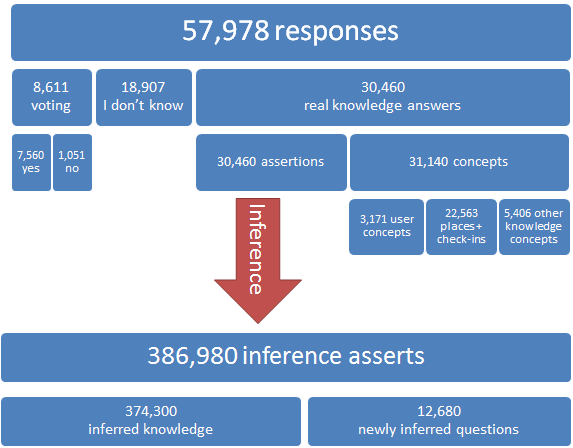
\includegraphics[width=1\textwidth]{figures/results.png}
	\caption{Graphical representation of collected answers (knowledge) and 
    distributions.}
	\label{fig:results}
\end{figure}

\begin{table}[h]
\centering
\caption{Examples of answered/asserted and inferred knowledge taken from
\emph{Curious Cat} KB.}
\label{tab:ccresultexamples}
\begin{tabular}{|c|l|l|}
	\hline
	\makecell[l]{\textbf{Type of the} \\ \textbf{collected knowledge}} & \textbf{Curious Cat Question} & \textbf{User Answer} \\
    \hline
    \textbf{User Concepts} &\makecell[l]{[automatic assert \\from registration]} & \makecell[l]{$is(User1,Person)$, \\ $name(User1,"Luka")$} \\
    \hline
    \textbf{Places + Check-ins} &\makecell[l]{[automatic assert \\from check-in \\ and Foursquare/\\Factual locations]} & \makecell[l]{$is(Place1,Restaurant)$, \\ $name(Place1,$\\"Pig'n Whistle"$)$} \\
     \hline
    \textbf{Other Concepts} &\makecell[l]{What did you order?} & \makecell[l]{Duck meat} \\
	\hline 
    \textbf{Real Knowledge 1} & Who is CEO of BMW? & Harald Kruger\\
	\hline
    \textbf{Real Knowledge 2} &\makecell[l]{What is the ticker symbol\\ of BMW?} & ABC \\
	\hline
    \textbf{voting(yes)} &\makecell[l]{Is it true that Herald Krueger\\ is the CEO of BMW company?} & yes \\
	\hline
    \textbf{voting(no)} &\makecell[l]{Is it true that ABC \\is the ticker symbol for BMW?} & no \\
	\hline
    \textbf{I don't know} &\makecell[l]{\_\_\_ and BMW are \\corporate competitors.} & I don't know \\
	\hline
    \textbf{Inferred knowledge 1} &\multicolumn{2}{l|}{$is(HeraldKrueger,Person)$} \\
	\hline
    \textbf{Inferred knowledge 2} &\multicolumn{2}{l|}{$anatomicalParts(HeraldKrueger,Hand)$} \\
	\hline
    \makecell[l]{\bfseries{Newly Inferred}\\ \bfseries{question}} &\multicolumn{2}{l|}{"What is Herald Krueger's age?"} \\
	\hline
\end{tabular}
\end{table}

While the resulting number and quality (\autoref{tab:baselines}, 
\autoref{tab:validity}) of assertions
shows that the presented approach can be successfully used for high quality KA,
we explored in more detail the contributions of specific characteristics of our
system and compare them to the baselines, to evaluate the ideas and claims
of the approach:
\begin{enumerate}
\item Using context to pro-actively drive the KA increases engagement and the 
chance of getting an answer (\autoref{section:evaluationContext})
\item Pre-existing knowledge and automated inference can be used to filter-out 
inconsistent answers and thus increase the quality of the acquired knowledge
\item Using newly acquired knowledge to further drive the KA process increases
the amount of acquired answers and reach of the system
\item Crowdsourcing additionally improves the results by filtering wrong but 
logically correct answers
\end{enumerate}

\section{Context and Pro-activity}
\label{section:evaluationContext}
\emph{Curious Cat} employs two contextual knowledge provision mechanisms. One 
is location based knowledge, such as, the type of current location, the time of
visit and the duration of stay. The second is internal knowledge that the 
system already knows about the user, such us, languages that the user speaks, 
food she likes, demographics data, interests, etc. In evaluation, we focused on
exploring benefits of using the location based context, since it is practically
impossible to disable internal knowledge without bigger changes in the system. 
Inferring without internal knowledge e.g., total removal of the personal 
knowledge would mean removal of almost all questions regarding people, animals,
human interests, etc., since these are general for human beings and to some 
extent to animals as well.

For the purpose of this experiment, we deliberately removed GPS location and 
connected mechanisms for derived knowledge for a duration of three months. We 
normalized the measures (assertions per user per day) for all experiments to 
level out the differences in the durations of experiments against a longer 
duration of fully operative system. The results are presented in 
\autoref{tab:ccresultscompare}. The columns in the table are organized as 
follows:

\begin{itemize}
\item first column contains measure name,
\item second column full data-set when using context (marked as C),
\item third is 100-day data-set when not using context (NC100),
\item and last is the normalized column with context (C100) which makes it 
possible to compare the context versus no context knowledge collection behavior (C100 vs NC100).
\end{itemize}

Since number of days and users is strongly correlated with the number of 
answers the system gets, and we only have the "No Context" data for 100 days 
(41 new users during that time and 45 active users), we normalized our 
"Context data" in such a way, that it matches the duration, new users and 
active users of \emph{NC100}. For this, we had to scan all the data-set 
day-by day with a range of 100-day window, where we looked at the number of new 
and active users in each of the 1264 sub-windows (number of all different 
100 day windows one can fit into 1264 days). In the whole data-set there was 
18 such 100-day windows, which can be directly compared to the \emph{NC100}. 
While the number of new users is fixed to 41, number of new assertions and 
active users still varies (min. 1,429, max. 9,279 new assertions and min. 47, 
max 61 active users). For this reason, we calculated the mean values of all 
18 windows which had the same number of new users as \emph{NC100}. Matching 
new users (instead of active users) was selected because new users are the
ones that contribute most of the assertions, since their interest winds down 
gradually. This can be seen on \autoref{fig:followups}. This is also the 
primary reason why (unintuitively) number of new assertions/day/active user 
(row 7 in {utoref{tab:ccresultscompare}) is higher without context 
(\emph{NC100}) than for  non-normalized data from experiment using context 
(\emph{C}).

\begin{table}[h]
\centering
\caption{Results of KA without context versus results while using location based context}
\label{tab:ccresultscompare}
\begin{tabular}{|l|l|l|l|}
	\hline
	\textbf{Measure}  & \makecell[l]{\textbf{With Location}\\\textbf{Context (C)}} & \makecell[l]{\textbf{Without Location}\\ \textbf{Context (NC100)}} &  \makecell[l]{\textbf{With Location}\\\textbf{Context 100}\\\textbf{days (C100)}}\\
    \hline
    1. Experiment duration & 1,364 days & 100 days & 100 days \\
    \hline
    2. Number of new assertions & 56,586 & 709 & 2,244 (+216.5\%) \\
    \hline
    \makecell[l]{3. Number of new assertions\\where user didn't\\ know the answer} & 18,380 (32\%) & 267 (38\%) & 667 (28.3\% = -9.7\%) \\
	\hline 
    \makecell[l]{4. Number of new \\assertions where \\user knew the answer}  &38,206 (68\%) & 442 (62\%) & 1,577 (71.7\% = +9.7\%) \\
	\hline
    \makecell[l]{5. Number of new \\assertions/day \\(all users) } & 42.1 & 7.1 & 22.4 (+215.5\%)\\
	\hline
    \makecell[l]{6. Number of new \\assertions/active user } & 90.3 & 15.7 & 44.2 (+181.5\%) \\
	\hline
    \makecell[l]{\textbf{7. Number of new}\\\textbf{assertions/day/active}\\\textbf{user}} & 0.07 & 0.16 & \textbf{0.44 (+175\%)} \\
	\hline
    \makecell[l]{8. Number of new \\concepts/day} & 3.7 & 0.4 & 2.4 (+85.2\%) \\
	\hline
    \makecell[l]{9. Number of new concepts \\ (excluding users and\\ locations)} & 4,925 & 36 & 243 (+85.2\%) \\
	\hline
    10. Number of active users & 625 & 45 & 49 \\
	\hline
    11. Number of new users & 625 & 41 & 41 \\
	\hline
\end{tabular}
\end{table}

The results of not using context show the decrease of raw new knowledge 
assertions from 56,568 to 709, which of course can be attributed to the fact 
that duration of experiment \emph{C} was much longer, or that it had more users
than \emph{NC100}. As described above, this is properly normalized in the 
column \emph{C100}, where the raw number of assertions raises to 2,244 
compared to only 709 when not using context (\textbf{context brings 217\% 
increase}).

While the majority of the increase is due to pro-active questions from 
\emph{Curious Cat}, which are linked to GPS clustering, some of the increase 
is also due to better targeting of the questions due to contextual data, 
since without the context only users are selecting the topics and the system 
doesnt have enough knowledge to successfully pick the most relevant next 
question. This is reflected in a slight increase in the proportion of the 
questions for which the user knows the answer (+9.7\% - row 4 in 
\autoref{tab:ccresultscompare}). This is independently of pro-active component 
which is mostly reflected in the raw number of assertions, while the 
knowing/not knowing ratio improvement is due to better targeting whatever 
question there was.

%subsection
\subsection{Consistency Checking}
\label{section:resultsConsistencyChecking}
Before the system accepts the answer from the user (as described in 
\autoref{section:consistency}), it converts it into logic and checks whether it 
is consistent with its current knowledge. If there is an inconsistency, it will 
reject the answer and thus prevent the wrong or contradicting knowledge to 
corrupt the KB and consequently the future KA process. The user then either has
to fix the answer, or convince the system that the answer is actually only a 
different name for the consistent knowledge. For example, if the user states 
that he ate a car in the restaurant, this is either wrong, or car is the name 
for some unknown food and not a vehicle.

Due to development process and time-line of the system, we only have logs and 
consequently insights on when/how the system rejected the answers due to 
inconsistency for 143 out of 1,472 days of the experiment duration. During 
this time, 148 users provided 23,543 answers and the system rejected 563 of 
them, so 22,980 of assertions went into the KB. Among the 563 rejections, 
some of them were repeating (user re-tries, or other users did the same 
mistake), so the system actually prevented 384 unique inconsistent answers.

%old table VII
\begin{table}[h]
\centering
\caption{Results of Consistency Checking}
\label{tab:resultsconsistencycheck}
\begin{tabular}{|l||l|l|}
	\hline
	\textbf{Measure}  &	 \makecell[l]{\textbf{Real data from}\\\textbf{the logs}} & \makecell[l]{\textbf{Extrapolation for}\\ \textbf{the full experiment}} \\
    \hline
    Number of new assertions & 22,980 & 57,978 days \\
    \hline
    \makecell[l]{Number of rejected assertions\\due to inconsistency} & 563 & 1420\\
    \hline
    \makecell[l]{\textbf{Percentage of rejected}\\\textbf{asserts}} & \textbf{2.45\%} & \textbf{2.45\%} \\	
	\hline 
    \makecell[l]{Number of unique rejected\\ asserts} & 384 & 968 \\
	\hline
    \makecell[l]{\textbf{Percentage of unique}\\ \textbf{rejected asserts}} & \textbf{1.67\%} & \textbf{1.67\%}\\
	\hline
    \makecell[l]{Number of new users } & 128 & 728 \\
	\hline
    \makecell[l]{Number of active users} & 148 & 728 \\
	\hline
    \makecell[l]{Experiment duration} & 143 days & 1472 days \\
	\hline
\end{tabular}
\end{table}

As presented in \autoref{tab:resultsconsistencycheck}, for every 100 valid 
answers users provided during the experiment, there were 2.45 answers which 
were rejected by the system due to being completely wrong or inconsistent. 
Because we only have logs for 143 days we had to extrapolate the number for the
overall experiment to get some estimation of how many bad assertions were 
prevented by the system throughout the whole experiment. The estimated number 
of rejected assertion system prevented overall is 1,420. Fore easier 
understanding, in \autoref{tab:rejectedconversation} are examples of the 
rejected assertions, together with the interaction that lead to the rejection.

%old table VIII
\begin{table}[h]
\centering
\caption{Conversation prior to rejected assertions}
\label{tab:rejectedconversation}
\begin{tabular}{|l|l|}
	\hline
	\textbf{CC}  & \textbf{User} \\
    \hline
    \multicolumn{2}{|c|}{\textbf{Example 1}} \\
    \hline
    \makecell[l]{Which social being has \\ Lagos as assets?} & hotel \\
    \hline
    \makecell[l]{By hotel do you mean\\ hotel (building)?} & yes\\
    \hline
    \multicolumn{2}{|l|}{\textbf{Rejected - building is not a social building}}\\
    \hline
    \multicolumn{2}{|c|}{\textbf{Example 2}} \\
    \hline
    \makecell[l]{Let's continue our\\ previous conversation \\ about going on a date.} & ok \\
    \hline
    \makecell[l]{All going on a date has\\ \_\_\_as a characteristic\\sub-event} & hello\\
    \hline
    \multicolumn{2}{|l|}{\textbf{Rejected - hello is a greeting, not an event.}}\\
    \hline
\end{tabular}
\end{table}

%subsection
\subsection{Additional knowledge as follow-up of newly acquired knowledge}
\label{section:followups}
As one of the more important features of our proposed system is its ability to 
use newly acquired knowledge to ask new things, we explored this functionality, 
comparing it to the baseline KA and consequently measuring the knowledge that 
was acquired as a consequence of prior acquisition. An example of such a 
follow up question or assertion is given in \autoref{tab:followupexample}.

%old table IX
\begin{table}[h]
\centering
\caption{Example of follow-up question and answers (new knowledge)}
\label{tab:followupexample}
\begin{tabular}{|c|l|}
	\hline
	1  & CC Asks: "What did you order?" \\
    \hline
    2 & User answers: "Meatloaf" \\
    \hline
    3 & \makecell[l]{CC asks a follow-up question: "One of the meatloaf\\ ingredients is \_\_\_". }\\
    \hline
    4 & User answers: "egg". \\
    \hline
\end{tabular}
\end{table}

The question number 3 in \autoref{tab:followupexample} is a "follow-up" question
since it is only asked when someone enters the previously unknown food concept. 
Answer under number 4 is a follow-up knowledge, since it was answered and given 
to the system only because someone created the concept of $Meatloaf$.

During the whole experiment the system collected and accepted \textbf{22,838 
answers}, which were a follow-up answer. This means that \textbf{39.4\%} of all
the knowledge we obtained was a direct consequence of the systems ability to 
generate new questions based on the already acquired knowledge.

The follow-up questions and answers are always a consequence of some new 
concept that enters the system. The 22,838 of answers are consequence of 
5,406 new concepts (not counting concepts of users themselves and locations 
they checked in), where the distribution of new knowledge/concept follows a 
long-tail distribution - a very small number of concepts triggered a big number
of follow-up knowledge (\autoref{fig:followups} - logarithmic scale).

\begin{figure}[H]
	\centering
		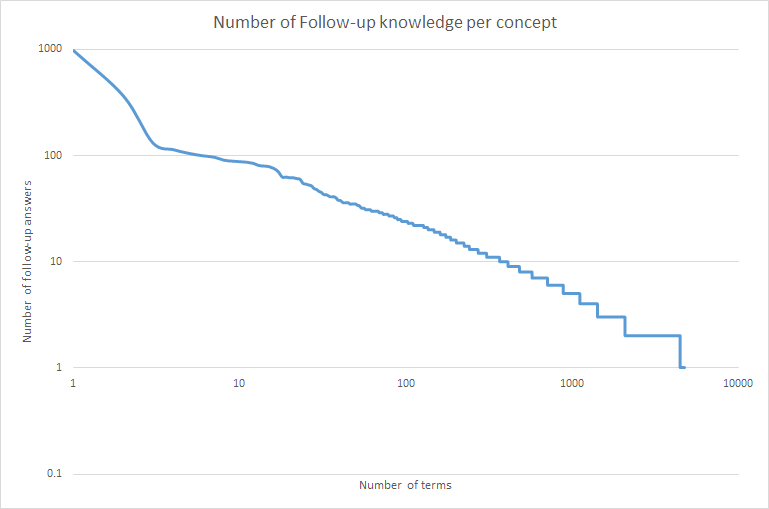
\includegraphics[width=1\textwidth]{figures/followupGraph.png}
	\caption{Long tail (logarithmic scale) distribution of follow-up answers per new concept}
	\label{fig:followups}
\end{figure}

%subsection
\subsection{Additional knowledge because of allowing cross-user cooperation}
\label{section:resultscross}
Similarly, as done for follow-up answers in \autoref{section:followups}, we can
check how much of the new knowledge came into the system due to its ability to 
share knowledge and questions cross-users. For this, we check the answers, 
where the initial concept was given to the system from a different user then the
follow up answer. From the example in \autoref{tab:followupexample} this would 
mean that the answer number 2 was given by $User1$ and then CC asks the 
question 3 and receives answer 4 from $User2$.

While for follow-up results, we have a complete log, due to changing the 
system, not all records have information about the original user who created 
the concept. We have his data only for 45 concepts out of 5406, excluding all 
user concepts and locations they checked-in. For these 45 concepts, 
we got additional 123 answers from other users.

%subsection
\subsection{Voting}
\label{section:resultsvoting}
The voting part of the system is, besides directly providing the answers, 
one of the main crowdsourcing components. As described in 
\autoref{section:crowdsourcing}, 
after the knowledge is acquired, the system can re-check with other users 
whether the assertion is true or not. This is done by presenting a question in 
the form: "Is it true that [assertion].", which can be answered with "yes" or 
"no". For example: "Is it true that Bornholmsk is a national language of 
Denmark?".

While the consistency check is performed automatically by the system, the 
answers that are manifestly inconsistent with the other content in the KB are 
stored only in the user specific part of the KB. Checking for truth of the 
knowledge is motivated by the fact that claims can be still be untrue even if 
they are consistent with the KB. From the Yes/No ratio, we can see that there 
are many more "Yes" votes than "No" votes, which hints that the answers the 
other users provide are mostly recognized as true by the crowd. 
This could be taken as a hint towards the precision of the truthfulness of the 
acquired knowledge. If we take into consideration that more users can vote for 
the same assertion, the effective precision of the knowledge measured this way 
can be estimated more accurately. The voting mechanism hides from the public 
knowledge base 97 of the assertions where the users were unable to agree on 
truth and 636 assertions which were voted as untrue by majority of the users.

%old table X
\begin{table}[h]
\centering
\caption{Crowd voting results}
\label{tab:votingresults}
\begin{tabular}{|l|l|}
	\hline
	\textbf{Measure}  & \textbf{Number} \\
    \hline
    All votes & 8,611 \\
    \hline
    Votes over unique asserts & 5,436 \\
    \hline
    Yes votes & 7,560 \\
    \hline
    No votes & 1,051 \\
    \hline
    Rejected answers & 636 \\
    \hline
    Accepted answers & 4,703 \\
    \hline
    Undecided answers & 97 \\
    \hline
\end{tabular}
\end{table}

If we look at some of the most rejected assertions, we can see assertions 
such as (more no votes than yes):
\begin{itemize}
\item $nationalLanguage (Denmark Bornholmsk)$ (3 yes, 9 no)
\item $typicalColorOfType (Automobile BlackColor)$ (3 yes, 9 no)
\item $is (CityOfCopenhagenDenmark Town)$ (0 yes, 4 no)
\item $subclass (Coffee-Beverage ArtificialMaterial)$ (3 yes, 9 no)
\item $soleMakerOfProductType (TelevisionSet PhilipsPetroleumCompany)$ (3 yes, 7 no)
\end{itemize}
And the most accepted assertions (more yes votes than no):
\begin{itemize}
\item $is (Denmark CountryWithOnlyOneTimeZone)$ (25 yes, 0 no)
\item $is (Food CollectionWithManySpecializzations)$ (23 yes, 0 no)
\item $sublcass (Food OrganicMaterial)$ (19 yes, 0 no)
\item $is (Food ProductTypeWithoutSoleMaker)$ (20 yes, 1 no)
\item $countryPhoneCode (Slovenia 386)$ (18 yes, 0 no)
\end{itemize}
And some of the undecided assertions (same number of yes and no votes):
\begin{itemize}
\item $subclass (IceCream Mixture)$ (2 yes, 2 no)
\item $characteristicProperSubeventTypes (CookingFood EatingEvent)$ (1 yes, 1 no)
\item $electronicDeviceMountingStyle (RearVideoPort DesktopComputer)$ (2 yes, 2 no)
\end{itemize}

%subsection
\subsection{User Stickiness Factor}
\label{section:stickiness}
To get an idea of how the users interacted with the system, we checked each of
them by the first and the last piece of knowledge they provided and measured 
the duration of days between these dates. This is a simple indicator of a 
stickiness - showing how many of the users only tried an application and then 
forgot about it and how many of them answered questions for longer. On
\autoref{fig:userstickiness} we can see the long-tail distribution of how long 
users stick with the application. About 25\% of the users stick with the 
system for more than just one-day testing. While most of the users (548) only 
tested the system for a day and did not use it further, 180 users stayed for a 
longer period of time. Among these, 117 used it for more than a week, 98 for 
more than two weeks, 69 for a month or more, 51 for more than two months and 
15 for more than a year.
\begin{figure}[H]
	\centering
		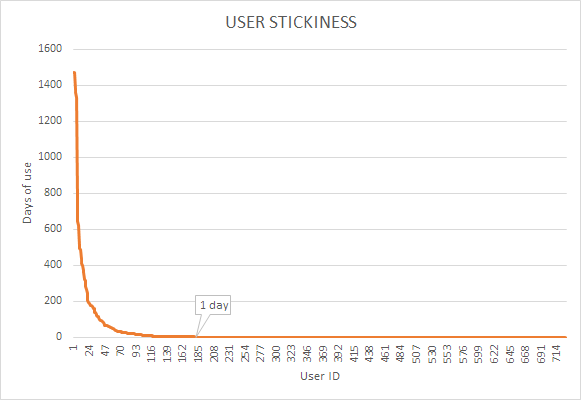
\includegraphics[width=1\textwidth]{figures/userStickiness.png}
	\caption{Distribution of usage duration for users}
	\label{fig:userstickiness}
\end{figure}

While this distribution is not too impressive for the commercial product, 
it is somehow expected for a research prototype without any updates and 
improvements for more than a year after it was built. It shows that the 
approach has potential and triggered interest in a decent number of the users, 
which indicates it could gain a lot of interest with a few improvements and 
obvious bug fixes.

%subsection
\subsection{Results Summary}
\label{section:resultssummary}
As a wrap-up of the result sections, \autoref{tab:baselines} shows the 
knowledge or quality contributions of particular system features and their 
appropriate baselines.

\begin{table}[h]
\centering
\caption{Contributions of separate system features and appropriate baselines}
\label{tab:baselines}
\begin{tabular}{|l|l|c|c|}
	\hline
	\makecell[c]{\textbf{System Feature}} & \makecell[c]{\textbf{Measure}} & \makecell[c]{\textbf{Baseline}} & \makecell[c]{\textbf{Proposed Approach}} \\
    \hline
	\multicolumn{4}{|c|}{\textbf{Knowledge Gathering}} \\    
    \hline
    Context and Proactivity & \makecell[l]{Number of gathered\\assertions/day} & 71 & \textbf{42.1} \\
     \hline
     \multirow{2}{10em}{Follow-up assertions (new knowledge due to already collected k.} & \makecell[l]{Number of gathered\\assertions} & 35,140 & \textbf{57,978} \\
	\cline{2-4}
																						       & \makecell[l]{Number of gathered \\assertions per concept} & 0 & \textbf{4.22} \\
	\hline 
	\multirow{2}{10em}{Cross-user assertions} & \makecell[l]{Number of gathered\\assertions\\(extrapolated)} & 43,920 & \textbf{57,978} \\
	\cline{2-4}
										     & \makecell[l]{Number of gathered\\assertions/concept} & 0 & \textbf{2.73} \\
	\hline
	\multicolumn{4}{|c|}{\textbf{Quality Control}} \\    
	\hline
	Consistency Checking & \makecell[l]{Number of removed\\bad answers} & 0 & \textbf{1420} \\
	\hline
	Crowd Voting & \makecell[l]{Number of removed\\bad answers} & 0 & \textbf{733}\\
	\hline
\end{tabular}
\end{table}

As the overall sanity check of the KB, we randomly picked 100 newly acquired 
assertions, and assessed them manually to see whether they were:
\begin{itemize}
\item Valid (in the sense of consistent with the KB here we expect 100\%)
\item True (in the sense of true in an interpretation based on our human world)
\item Useful (useful for a potential user, or for the inference engine in 
producing suggestions, validations, new questions)
\end{itemize}

The counts are presented in \autoref{tab:validity}. As expected all the 
assertions are 
valid, 96\% of them are true and 95\% are useful. This can be used as an 
estimate of the knowledge that we acquired through the proposed approach.

%old table XII
\begin{table}[h]
\centering
\caption{Results of manual evaluation on 100 randomly picked assertions}
\label{tab:validity}
\begin{tabular}{|c|c|c|}
	\hline
	\textbf{Valid} & \textbf{True} & \textbf{Useful} \\
    \hline
	100 & 96 & 95 \\    
    \hline
\end{tabular}
\end{table}

The results of this counting are not surprising, since the system does not allow 
manifestly inconsistent assertions, and the crowdsourcing mechanism already 
weeded out most of the untrue examples. There were four untrue assertions in 
the sample, which expose three potential problems:
\begin{enumerate}
\item One error was because the price of the coffee changed since the last 
check with the users  the stored knowledge was obsolete.
\item There were two concepts with exactly the same name and were both 
subclasses of $Organization$, so the users and also the system did not manage to 
distinguish them and picked the wrong one. For users, everything seemed 
perfectly correct even though a logical error resulted.
\item Twice the user entered a complex sentence instead of a name of the 
concept and that forced the system to create a concept with that name (a
consequence of disabled SCG (see \autoref{section:cycnl}).
\end{enumerate}

Looking more in details of the usefulness of the retrieved knowledge, there 
were two answers, which related to the internal KB mechanism (how to handle 
events) and were thus not really useful for the end user. The remaining there 
were mostly too specific and not really useful in general, such as the name of 
the spider the user has in the corner of a room.
